\documentclass[11pt]{scrartcl}
\usepackage[T1]{fontenc}
\usepackage[a4paper, left=3cm, right=2cm, top=2cm, bottom=2cm]{geometry}
\usepackage[activate]{pdfcprot}
\usepackage[ngerman]{babel}
\usepackage[parfill]{parskip}
\usepackage[utf8]{inputenc}
\usepackage{kurier}
\usepackage{amsmath}
\usepackage{amssymb}
\usepackage{xcolor}
\usepackage{epstopdf}
\usepackage{txfonts}
\usepackage{fancyhdr}
\usepackage{graphicx}
\usepackage{prettyref}
\usepackage{hyperref}
\usepackage{eurosym}
\usepackage{setspace}
\usepackage{units}
\usepackage{eso-pic,graphicx}
\usepackage{icomma}
\usepackage{pdfpages}

\definecolor{darkblue}{rgb}{0,0,.5}
\hypersetup{pdftex=true, colorlinks=true, breaklinks=false, linkcolor=black, menucolor=black, pagecolor=black, urlcolor=darkblue}



\setlength{\columnsep}{2cm}


\newcommand{\arcsinh}{\mathrm{arcsinh}}
\newcommand{\asinh}{\mathrm{arcsinh}}
\newcommand{\ergebnis}{\textcolor{red}{\mathrm{Ergebnis}}}
\newcommand{\fehlt}{\textcolor{red}{Hier fehlen noch Inhalte.}}
\newcommand{\betanotice}{\textcolor{red}{Diese Aufgaben sind noch nicht in der Übung kontrolliert worden. Es sind lediglich meine Überlegungen und Lösungsansätze zu den Aufgaben. Es können Fehler enthalten sein!!! Das Dokument wird fortwährend aktualisiert und erst wenn das \textcolor{black}{beta} aus dem Dateinamen verschwindet ist es endgültig.}}
\newcommand{\half}{\frac{1}{2}}
\renewcommand{\d}{\, \mathrm d}
\newcommand{\punkte}{\textcolor{white}{xxxxx}}
\newcommand{\p}{\, \partial}
\newcommand{\dd}[1]{\item[#1] \hfill \\}

\renewcommand{\familydefault}{\sfdefault}
\renewcommand\thesection{}
\renewcommand\thesubsection{}
\renewcommand\thesubsubsection{}


\newcommand{\themodul}{Optische Technologie}
\newcommand{\thetutor}{Prof. Rateike}
\newcommand{\theuebung}{Übung 2}

\pagestyle{fancy}
\fancyhead[L]{\footnotesize{C. Hansen}}
\chead{\thepage}
\rhead{}
\lfoot{}
\cfoot{}
\rfoot{}

\title{\themodul{}, \theuebung{}, \thetutor}


\author{Christoph Hansen \\ {\small \href{mailto:chris@university-material.de}{chris@university-material.de}} }

\date{}


\begin{document}

\maketitle

Dieser Text ist unter dieser \href{http://creativecommons.org/licenses/by-nc-sa/4.0/}{Creative Commons} Lizenz veröffentlicht.

\textcolor{red}{Ich erhebe keinen Anspruch auf Vollständigkeit oder Richtigkeit. Falls ihr Fehler findet oder etwas fehlt, dann meldet euch bitte über den Emailkontakt.}

\tableofcontents


\newpage



\section{Aufgabe 1}


\begin{align*}
I \sim \frac{\sin^2\left( \frac{N \phi}{2} \right)}{\sin\left( \frac{\phi}{2} \right)} \underset{\phi \rightarrow 0, \ \sin(x) \approx x}{\longrightarrow} \frac{\left( \frac{N \phi}{2} \right)^2}{\frac{\phi}{2}} = N^2 
\end{align*}


\section{Aufgabe 2}

nicht lösbar


\section{Aufgabe 3}


\begin{figure}[h]
	\centering
	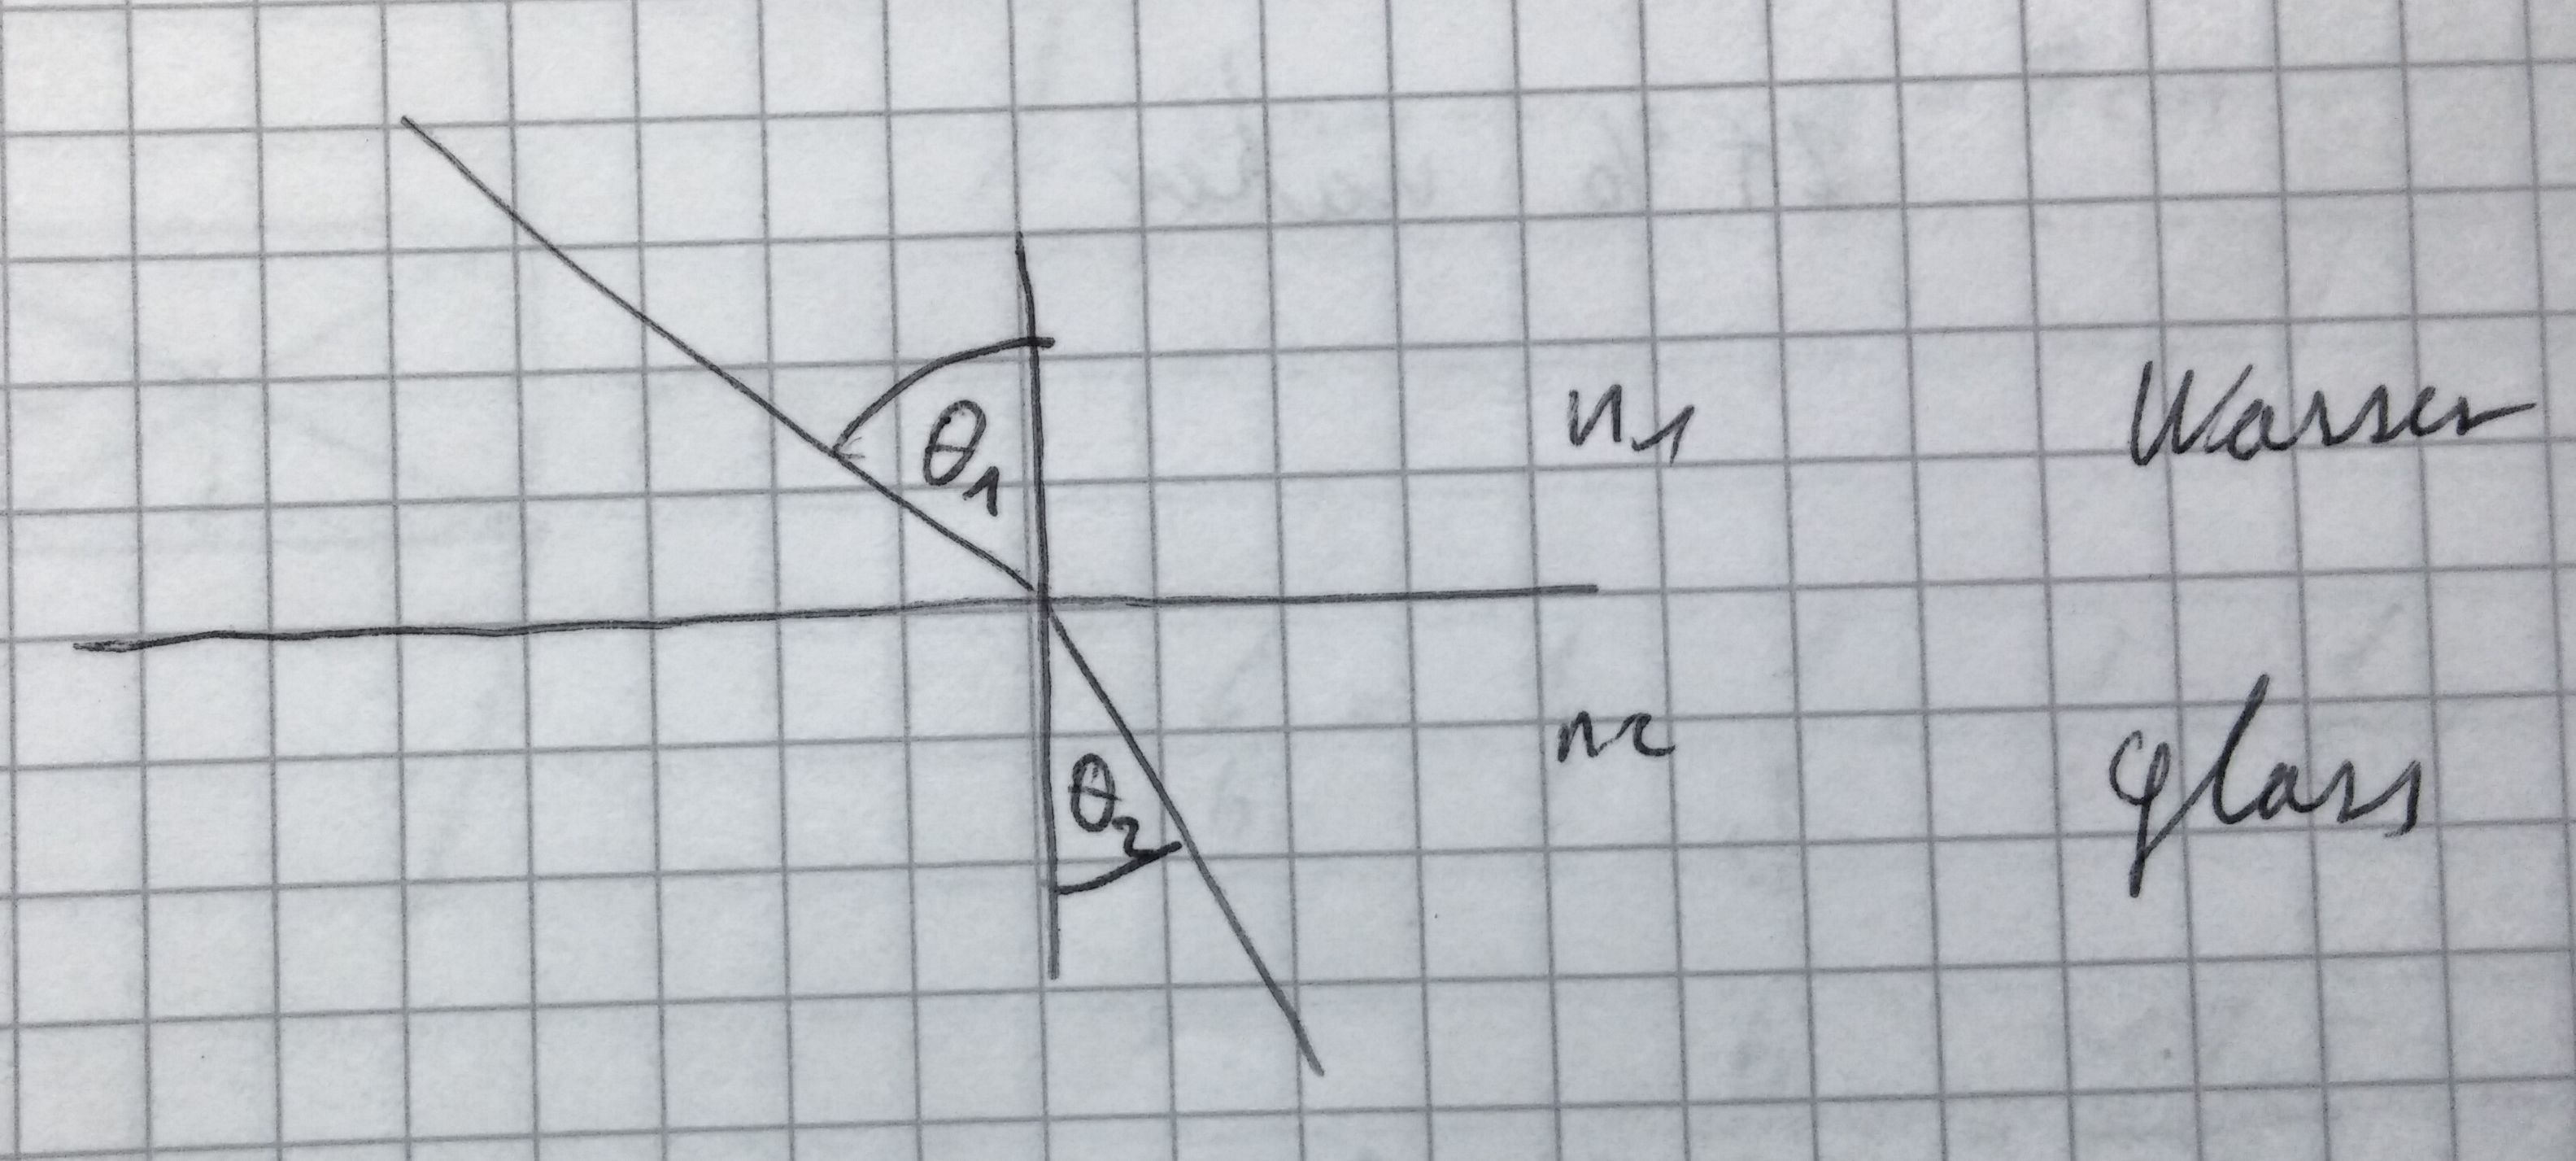
\includegraphics[scale=0.6]{A3_1.jpg}	
\end{figure}

\begin{align*}
I(\theta) &= \frac{\sin^2\left( \frac{\pi b \sin(\theta)}{\lambda} \right)}{\left( \frac{\pi b \sin(\theta)}{\lambda} \right)^2}
\intertext{Im ersten Minimum gilt:}
\pi &= \frac{\pi b \sin(\theta)}{\lambda}
\intertext{Da wir kleine Winkel betrachten gilt auch:}
\tan(\theta) &= \theta = \sin(\theta) = \frac{\lambda}{b}
\intertext{Wir definieren $\Delta x$ als den Abstand vom zentralen Maximum zum ersten Minumum:}
\Delta x &= L \cdot \frac{\lambda}{b}
\end{align*}


\newpage

\section{Aufgabe 4}

Die Intensität ist hier:

\begin{align*}
I(\theta) \sim \left[ \frac{2 j_1 \cdot \left( \pi d \cdot \frac{\sin(\theta)}{\lambda} \right)}{\pi d \frac{\sin(\theta)}{\lambda}} \right]^2
\intertext{Der erste dunkle Ring entspricht nun der ersten Nullstelle von $j_1$. Aus der Vorlesund wissen wir das dies bei $x = 1,22 \pi$ der Fall ist:}
1,22 \pi &= \pi d \cdot \frac{\sin(\theta)}{\lambda} \\
\Leftrightarrow \sin(\theta) &= 1,22 \cdot \frac{\lambda}{d} \approx \theta
\end{align*}

Dabei ist $d$ der Durchmesser des Lochs. Ab hier geht es dann weiter wie in A3.



\section{Aufgabe 5}

Das Beugungsbild sieht ungefähr so aus:

\begin{figure}[h]
	\centering
	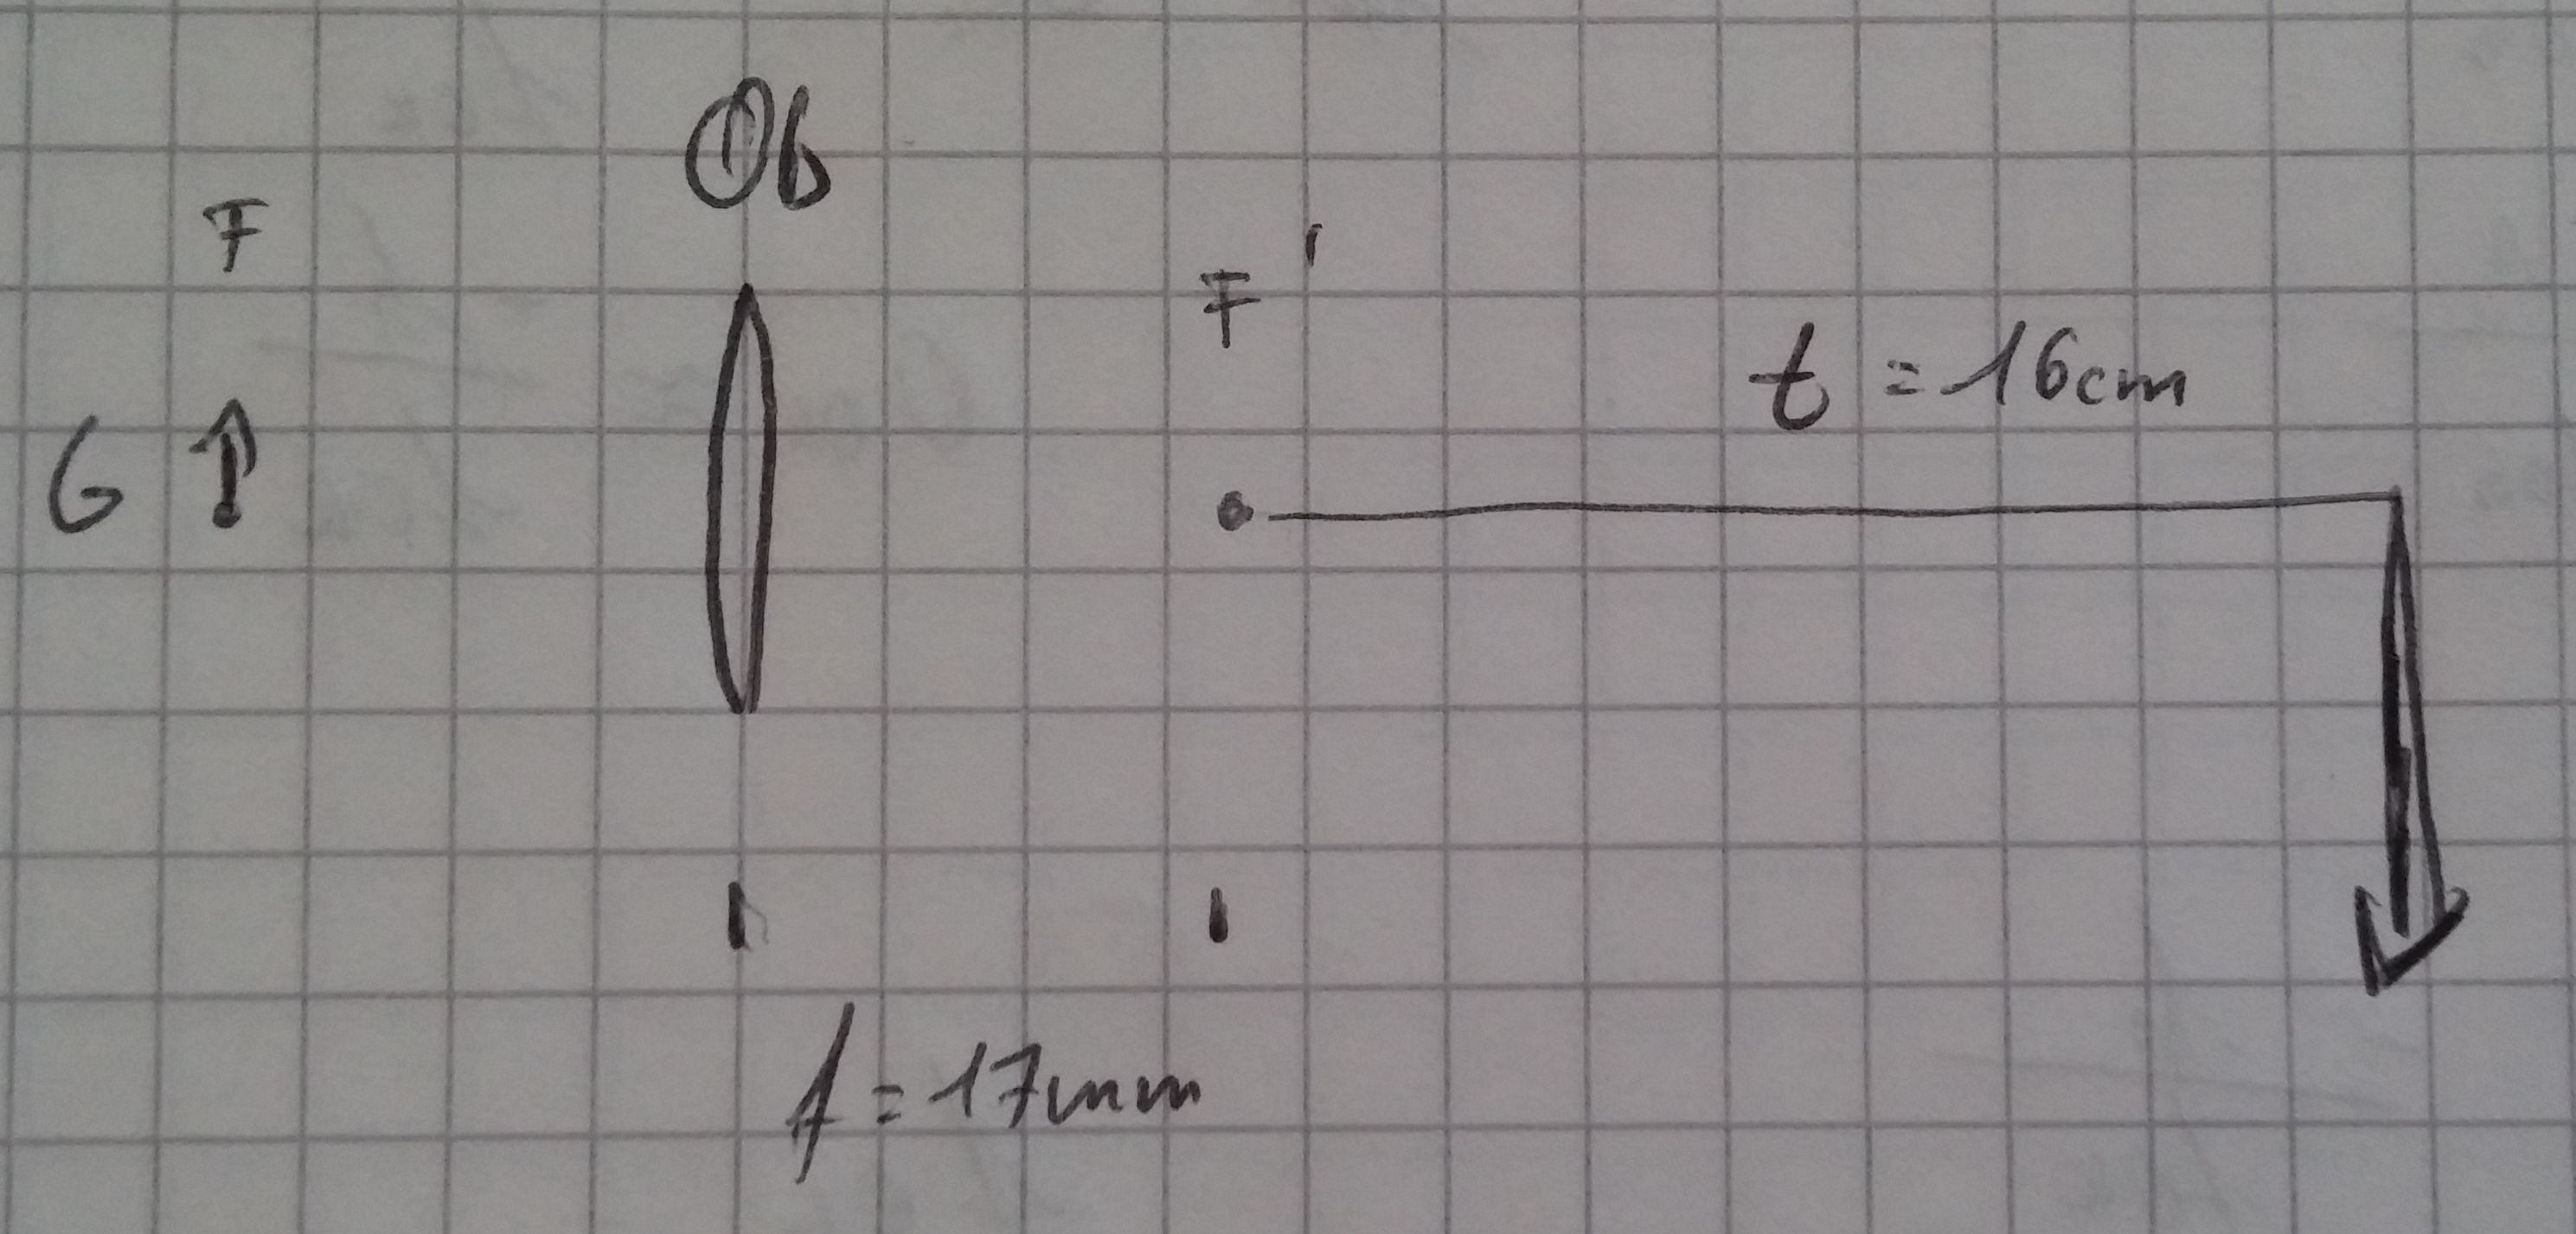
\includegraphics[scale=0.43]{A5_1.jpg}	
\end{figure}


Dabei gelten die folgenden Zusammenhänge:

\begin{align*}
\intertext{Maxima und in Phase}
d \cdot sin(\theta) &= N \cdot \lambda 
\intertext{Minima:}
d \cdot sin(\theta) &= \left( N + \half \right) \cdot \lambda 
\end{align*}





















\end{document}